\chapter{Materials and Methods}
\label{chap:methods}
This chapter presents the methodological design of the proposed system in two stages. First, we introduce DynaDA3 as the dense reconstruction module, which adapts the DA3 framework to endoscopic scenes and enhances the geometric prediction with dynamic occlusion filtering. Building upon this reconstruction module, we then present DynaDA3-SLAM, which extends DynaDA3 with SLAM functionality to support real-time localization, mapping, and navigation in monocular surgical environments. Figure~\ref{fig:DynaDA3_architecture} provides an overview of the DynaDA3 architecture, while Figure~\ref{fig:DynaDA3_slam_architecture} summarizes the overall DynaDA3-SLAM pipeline.
% 本章从两个阶段介绍本文方法的整体设计。
% 首先介绍 DynaDA3 作为稠密重建模块，
% 它将 DA3 框架适配到内窥镜场景，并通过动态遮挡过滤增强几何预测。
% 在此基础上，进一步介绍 DynaDA3-SLAM，
% 即将 DynaDA3 扩展为支持单目手术场景实时定位、建图与导航的 SLAM 系统。
% 图~\ref{fig:DynaDA3_architecture} 和图~\ref{fig:DynaDA3_slam_architecture}
% 分别给出了 DynaDA3 和 DynaDA3-SLAM 的整体架构示意。
%%%%%%%%%%%%%%%%%%%%%%%%%%%%%%%%%%%%%%%%%%%%%%%%%%%%%%%%
\section{DynaDA3}
\label{sec:network_architecture} 
%%%%%%%%%%%%%%%%%%%%%%%%%%%%%
\subsection{Preprocessing}             
Endoscopic video data typically presents unique visual challenges compared to standard datasets, including a circular field of view (FOV) surrounded by black borders and non-uniform illumination characterized by specular reflections and underexp§osed peripheral regions. 
To ensure the robustness of the subsequent network inference, we apply a two-stage preprocessing pipeline comprising region of interest cropping and illumination correction.
% 与常规视觉数据相比，内窥镜视频具有更特殊的输入特性，
% 包括黑色边框包围的圆形视场，以及由高光反射和边缘欠曝光带来的不均匀照明。
% 为了提高后续网络推理的稳定性，
% 本文采用两阶段预处理流程，包括感兴趣区域裁剪和光照校正。

\subsubsection{Region of Interest Cropping}
To eliminate irrelevant information from the black borders and focus the network's attention on the surgical site, we employ a fixed-ratio cropping strategy. As implemented in our pipeline, we extract a square region from the original video frames. The crop size is determined dynamically based on the image height:
% 为了去除黑色边界带来的无关信息，并使网络关注手术区域，
% 本文采用固定比例的裁剪策略。
% 在具体实现中，从原始视频帧中提取一个方形区域，
% 裁剪尺寸根据图像高度动态确定。
\begin{center}
    $ S_{crop} = H_{img} \times \lambda_{crop} $
\end{center}
where $H_{img}$ is the height of the original frame and $\lambda_{crop}$ is a scaling factor (experimentally set to 0.65 for the C3VD2 dataset) to cover the relevant endoscopic view. The crop window is centered horizontally with a learned offset to align with the endoscopic center, and positioned vertically to retain a balanced view of the surgical cavity, discarding the extreme upper and lower black margins.
% 其中，$H_{img}$ 表示原始图像高度，
% $\lambda_{crop}$ 是控制裁剪范围的比例系数，
% 在 C3VD2 数据集上实验设为 0.65。
% 裁剪窗口在水平方向以学习得到的偏移量对准内窥镜中心，
% 在垂直方向保留较均衡的手术腔视野，
% 从而去除上下边缘大面积的黑色无效区域。

\subsubsection{Illumination Correction}
To reduce the impact of severe specular highlights in endoscopic images, we adopt a learning-based two-stage highlight suppression strategy inspired by the method of Li et al.~\cite{li2025twostagehighlight}. In contrast to heuristic brightness adjustment, this approach explicitly detects highlight regions and then restores the corrupted appearance using context-aware inpainting, which is more suitable for surgical scenes where saturated reflections frequently obscure tissue texture.
% 为减弱内窥镜图像中强烈镜面高光的影响，
% 本文采用受 Li 等人方法启发的学习式两阶段高光抑制策略。
% 与启发式亮度调整不同，该方法先显式检测高光区域，
% 再利用结合上下文的修复网络恢复受损外观，
% 更适合组织纹理常被饱和反射遮挡的手术场景。

In the first stage, the cropped RGB frame is processed by a Hierarchical Feature Attention Network (HFA-Net), which predicts a binary highlight mask $\mathbf{M}$ together with a coarse de-highlighted image $\mathbf{D}_{\text{coarse}}$. Following the improved dichromatic reflection formulation in~\cite{li2025twostagehighlight}, the coarse image is modeled as
% 在第一阶段，裁剪后的 RGB 图像被送入层次化特征注意力网络 HFA-Net，
% 同时预测二值高光掩码 $\mathbf{M}$ 和粗略去高光图像 $\mathbf{D}_{\text{coarse}}$。
% 按照改进后的二色反射模型，
% 粗去高光结果可写为下式。
\begin{center}
    $\displaystyle \mathbf{D}_{\text{coarse}} = \mathbf{I}\odot(1-\mathbf{M}) + (\mathbf{I}-\mathbf{S})\odot\mathbf{M},$
\end{center}
where $\mathbf{I}$ denotes the input image, $\mathbf{S}$ is the estimated specular component, and $\odot$ denotes element-wise multiplication. This stage focuses on accurate localization of highlight regions and an initial suppression of saturated reflections.
% 其中，$\mathbf{I}$ 表示输入图像，
% $\mathbf{S}$ 表示估计得到的镜面反射分量，
% $\odot$ 表示逐元素乘法。
% 该阶段的重点在于准确定位高光区域，
% 并对饱和反射进行初步抑制。

The HFA-Net backbone combines hierarchical attention and local feature refinement to better distinguish true specular highlights from naturally bright tissue regions. In particular, the network integrates spatial-shift segmented attention, dual-flow attention, multi-scale feature fusion, and partial mask convolution, enabling both precise highlight detection and coarse removal~\cite{li2025twostagehighlight}. This is important in endoscopic imagery, where simple thresholding often confuses wet tissue reflections with normal bright anatomical structures.
% HFA-Net 主干通过结合层次化注意力与局部特征精化，
% 更好地区分真实镜面高光与本身较亮的组织区域。
% 具体而言，网络融合了空间位移分段注意力、双流注意力、
% 多尺度特征融合以及局部掩码卷积，
% 从而同时实现精确的高光检测和粗去除。
% 这一点对内窥镜图像尤其重要，
% 因为简单阈值法常常会把湿润组织反光误判为普通亮结构。

In the second stage, the coarse result is refined using a large-mask inpainting model based on LaMa. Before inpainting, the predicted highlight mask is morphologically dilated to enlarge the corrupted region and expose a wider contextual neighborhood. The dilated mask together with $\mathbf{D}_{\text{coarse}}$ are then fed into the inpainting network, which reconstructs texture-consistent tissue appearance and produces smoother transitions between corrected and unmodified regions. Compared with direct filtering, this two-stage design better preserves structural continuity around highlight boundaries and reduces visible artifacts in restored areas~\cite{li2025twostagehighlight}.
% 在第二阶段，基于 LaMa 的大掩码修复网络对粗结果进一步细化。
% 在修复之前，首先对预测得到的高光掩码进行形态学膨胀，
% 以扩大受损区域并暴露更宽的上下文邻域。
% 随后将膨胀后的掩码与 $\mathbf{D}_{\text{coarse}}$ 一同输入修复网络，
% 重建纹理一致的组织外观，并使修复区域与未修改区域之间的过渡更平滑。
% 相比直接滤波，这种两阶段设计更能保持高光边界附近的结构连续性，
% 并减少修复结果中的可见伪影。

The final output of this preprocessing step is a highlight-suppressed RGB image that is used as the input to the DynaDA3 network. By reducing saturated reflections before geometric inference, this step improves the visibility of tissue texture and helps stabilize subsequent depth, ray, and confidence predictions.
% 该预处理阶段的最终输出是去除高光后的 RGB 图像，
% 并将其作为 DynaDA3 网络的输入。
% 通过在几何推理之前抑制饱和反射，
% 这一过程提高了组织纹理的可见性，
% 并有助于稳定后续深度、射线和置信度预测。
%%%%%%%%%%%%%%%%%%%%%%%%%%%%%
\subsection{Architecture}
\label{subsec:architecture}

\begin{figure}[htbp]
    \centering
    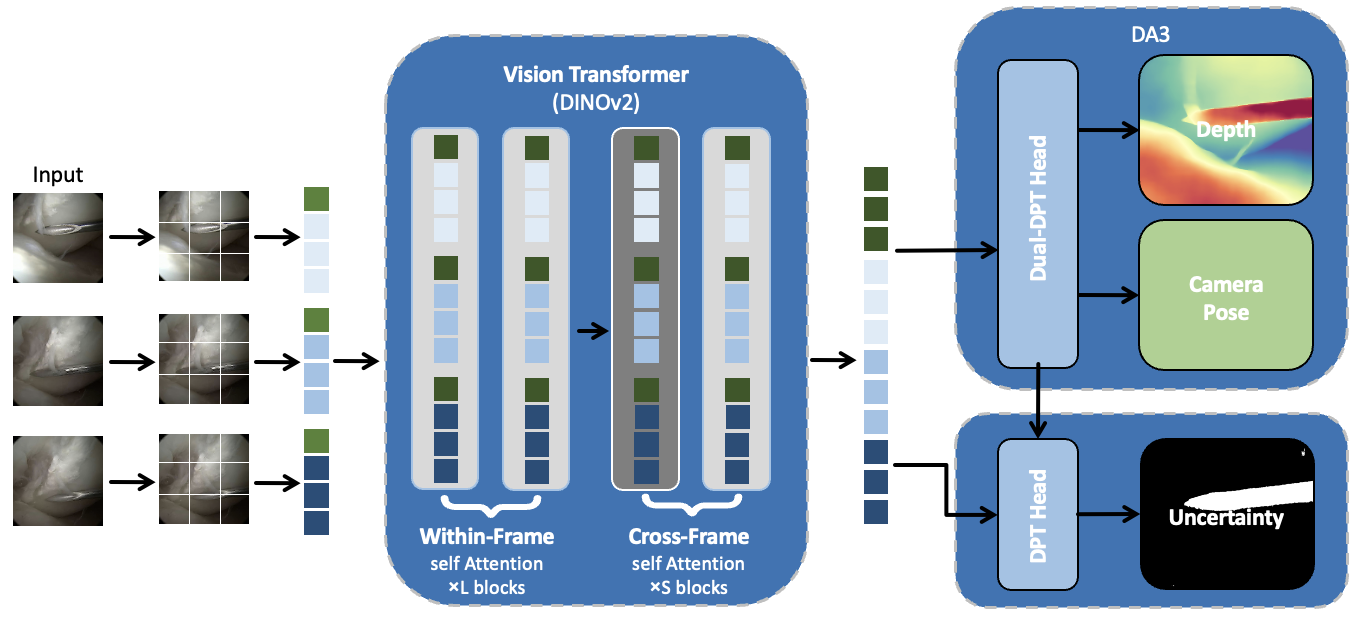
\includegraphics[width=0.95\textwidth]{4_images/3_Materials&Methods/DynaDA3.png}
    \caption[DynaDA3 architecture]{Overview of the proposed DynaDA3 architecture. The pipeline combines preprocessing, frozen DA3-based geometric prediction, and a trainable DPT head for dynamic occlusion filtering.}
    \label{fig:DynaDA3_architecture}
\end{figure}

As illustrated in Figure~\ref{fig:DynaDA3_architecture}, the DynaDA3 architecture is constructed upon the Depth Anything V3 (DA3) framework~\cite{lin2025da3}. The system is composed of two primary stages: a frozen geometric foundation model for feature extraction and geometric estimation, and a trainable DPT Head for dynamic occlusion segmentation.
% 如图~\ref{fig:DynaDA3_architecture} 所示，
% DynaDA3 架构建立在 Depth Anything V3 (DA3) 框架之上。
% 整个系统由两个主要部分构成：
% 一个冻结的几何基础模型用于特征提取与几何估计，
% 以及一个可训练的 DPT Head 用于动态遮挡分割。

\subsubsection*{DA3 Backbone and Geometric Outputs}
The backbone of DynaDA3 utilizes the DINOv2 ViT-Large encoder initialized with DA3 pre-trained weights. To preserve the robust zero-shot geometric generalization capabilities of the foundation model, the backbone parameters are frozen during training. 
The input image is processed to extract multi-scale semantic tokens from specific transformer layers (e.g., layers 11, 15, 19, and 23 for the ViT-L configuration). Simultaneously, the original DA3 Dual DPT Head processes these tokens to predict dense Depth and Ray maps. Crucially, we also extract the pixel-wise \textbf{Confidence Map} ($\mathbf{C}$) generated by the geometric head. This confidence map serves as a proxy for geometric uncertainty, where regions of low confidence often correspond to dynamic surgical tools, smoke, or specular reflections that violate multi-view consistency.
% DynaDA3 的主干采用以 DA3 预训练权重初始化的 DINOv2 ViT-Large 编码器。
% 为保留该基础模型较强的零样本几何泛化能力，
% 在训练过程中主干参数保持冻结。
% 输入图像会从特定的 transformer 层中提取多尺度语义 token，
% 同时由原始 DA3 的 Dual DPT Head 预测稠密深度图和射线图。
% 此外，本文还提取几何头输出的逐像素置信度图 $\mathbf{C}$。
% 该置信度图被视作几何不确定性的代理，
% 其中低置信度区域往往对应动态器械、烟雾或破坏多视图一致性的高光反射。

\subsubsection*{DPT Head}
% 这里的架构看还要不要优化
tobe optimized

%%%%%%%%%%%%%%%%%%%%%%%%%%%%%
\subsection{Training}
The training process is divided into two stages to ensure stability. First, we freeze the DINOv2 backbone and the pre-trained DA3 heads, fine-tuning only the DPT Head on the [Dataset Name] dataset. The occlusion segmentation is supervised using a combination of weighted binary cross-entropy (BCE) loss and Dice loss:
% 为保证训练稳定性，整个训练过程被划分为两个阶段。
% 第一阶段冻结 DINOv2 主干和预训练 DA3 头部，
% 仅在目标数据集上微调 DPT Head。
% 动态遮挡分割采用加权二值交叉熵损失和 Dice 损失的组合进行监督。
\begin{center}
    $ \mathcal{L}_{motion} = \lambda_{bce}\mathcal{L}_{BCE} + \lambda_{dice}\mathcal{L}_{Dice}, $
\end{center}
where $\lambda$ represents the balancing coefficients. Once the DPT Head converges, we unfreeze the entire network for joint end-to-end fine-tuning, ensuring the geometric predictions and motion-aware masking are mutually optimized for the surgical domain.
% 其中，$\lambda$ 表示不同损失项之间的平衡系数。
% 在 DPT Head 收敛之后，
% 进一步解冻整个网络进行端到端联合微调，
% 使几何预测与运动感知掩码能够共同适应手术场景。
%%%%%%%%%%%%%%%%%%%%%%%%%%%%%%%%%%%%%%%%%%%%%%%%%%%%%%%%%
\section{DynaDA3-SLAM}
\label{sec:slam_framework}
Building on the filtered geometry produced by DynaDA3, we further construct DynaDA3-SLAM as the real-time localization and navigation module of the overall system. In contrast to classical sparse-feature SLAM, the proposed method is formulated as a submap-level dense point-cloud SLAM pipeline. The system processes the input video in a fixed loop: incoming frames are read and optionally filtered by keyframe selection, a current submap with temporal overlap is formed, the learned front-end predicts geometry and prepares loop candidates, relative constraints are inserted into a global graph, the graph is optimized, and the refined global transforms are written back to the map. Consequently, the global optimization variables are submaps rather than individual frame poses, while the dense local geometry inside each submap is primarily provided by the learned front-end.
% 在 DynaDA3 提供过滤后几何结果的基础上，
% 本文进一步构建 DynaDA3-SLAM 作为整体系统中的实时定位与导航模块。
% 与经典逐帧稀疏特征 SLAM 不同，
% 该方法被建模为一种子图级的稠密点云 SLAM 流程。
% 系统按照固定循环工作：
% 读取输入帧、可选地进行关键帧筛选、构建带时间重叠的当前子图、
% 由学习式前端预测几何并准备回环候选、向全局图中加入相对约束、
% 执行图优化，并将优化后的全局变换写回地图。
% 因而，后端全局优化的变量是子图而非单帧位姿，
% 而每个子图内部的稠密局部几何主要由学习式前端提供。

\begin{figure}[htbp]
    \centering
    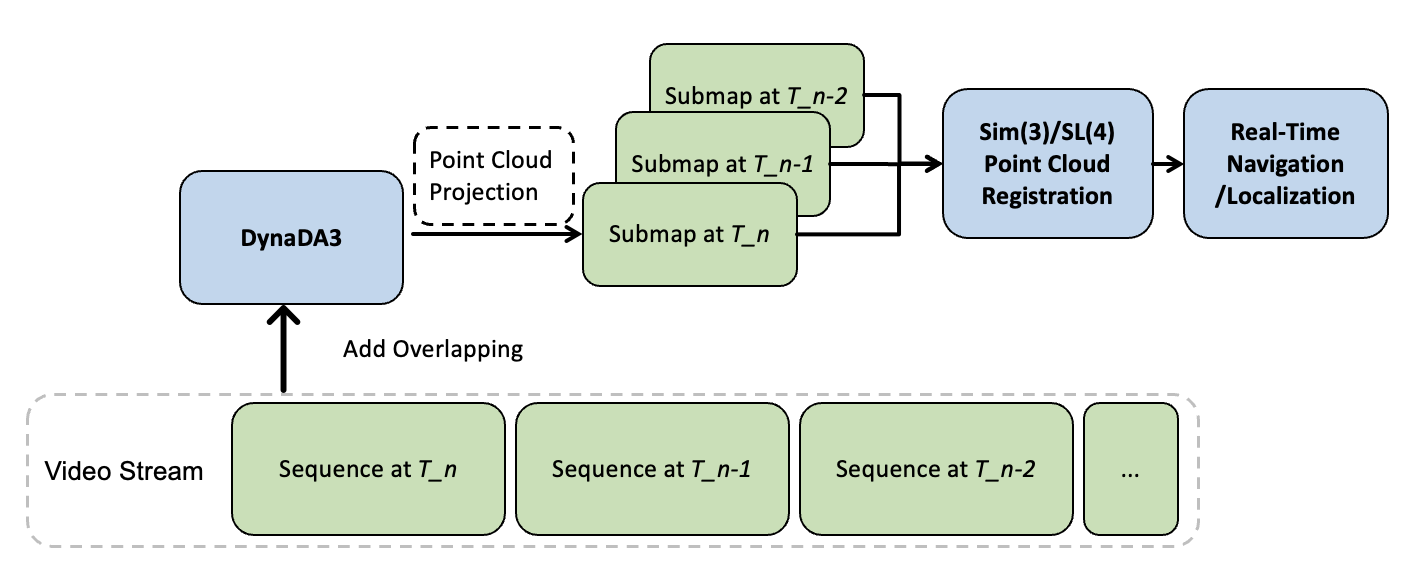
\includegraphics[width=0.95\textwidth]{4_images/3_Materials&Methods/DynaDA3-SLAM.png}
    \caption[DynaDA3-SLAM architecture]{Overview of the proposed DynaDA3-SLAM architecture. The system builds on DynaDA3 outputs and integrates local submap construction, projective alignment, and global optimization for monocular endoscopic SLAM.}
    \label{fig:DynaDA3_slam_architecture}
\end{figure}
%%%%%%%%%%%%%%%%%%%%%%%%%%%%%
\subsection{System Principle and Core Components}
As illustrated in Figure~\ref{fig:DynaDA3_slam_architecture}, DynaDA3-SLAM is organized around a small number of tightly coupled modules. The class \texttt{Solver} acts as the main controller and coordinates batched inference, submap construction, inter-submap registration, loop-closure insertion, optimization, and visualization. The learned front-end is encapsulated in \texttt{DynaDA3}, which internally calls Depth Anything 3 to predict dense depth, confidence, camera extrinsics, and camera intrinsics, while additionally invoking the uncertainty head to suppress dynamic or geometrically unreliable regions. The module \texttt{UncertaintyDPT} performs this binary segmentation by fusing depth, confidence, depth gradients, and backbone features. For frame selection, \texttt{FrameTracker} evaluates motion magnitude from Shi--Tomasi corners tracked by pyramidal Lucas--Kanade optical flow. Loop detection is handled by \texttt{ImageRetrieval}, which extracts global descriptors with SALAD/DINOv2. The class \texttt{Submap} stores local dense geometry, local camera poses, colors, confidences, masks, and the submap-to-world transform, whereas \texttt{GraphMap} manages the collection of all submaps and writes optimized transforms back to the map. Finally, \texttt{PoseGraph} provides the back-end graph optimization.
% 如图~\ref{fig:DynaDA3_slam_architecture} 所示，
% DynaDA3-SLAM 由一组紧密耦合的核心模块构成。
% 其中，\texttt{Solver} 作为总控模块，
% 负责批量推理、子图构建、子图间配准、回环约束添加、优化与可视化更新。
% 学习式前端由 \texttt{DynaDA3} 封装，
% 内部调用 Depth Anything 3 预测稠密深度、置信度、相机外参与内参，
% 并结合不确定性分支抑制动态或几何上不可靠的区域。
% \texttt{UncertaintyDPT} 通过融合深度、置信度、深度梯度和主干特征完成二值分割；
% \texttt{FrameTracker} 用于关键帧筛选；
% \texttt{ImageRetrieval} 用于回环检测前端；
% \texttt{Submap} 保存局部稠密几何、局部相机位姿、颜色、置信度、掩码和子图到全局的变换；
% \texttt{GraphMap} 管理所有子图并负责优化结果回写；
% \texttt{PoseGraph} 则提供后端图优化能力。

\subsection{Image Scheduling and Keyframe Selection}
The video stream is first ordered by frame index and then processed in windows of size \texttt{submap\_size + overlapping\_window\_size}. After a submap has been processed, only the tail overlap is retained as the starting segment of the next window. This overlap mechanism guarantees geometric continuity between neighboring submaps while keeping the memory footprint bounded. Before a frame is accepted into the current processing batch, the system may optionally apply keyframe selection. Specifically, \texttt{FrameTracker} detects Shi--Tomasi corners and tracks them with pyramidal Lucas--Kanade optical flow. The average pixel displacement of the surviving tracks is used as a disparity measure, and the frame is retained only if the motion exceeds a predefined threshold. In this way, the system avoids feeding highly redundant frames into the front-end while still preserving sufficient parallax for dense reconstruction and registration.
% 输入视频首先按照帧编号排序，
% 随后以大小为 \texttt{submap\_size + overlapping\_window\_size} 的窗口进行处理。
% 每个子图处理完成后，仅保留末尾的 overlap 帧作为下一个窗口的起点。
% 这种重叠机制在控制内存占用的同时，
% 保证了相邻子图之间的几何连续性。
% 在帧被送入当前处理批次之前，系统还可以选择性地进行关键帧筛选。
% 具体而言，\texttt{FrameTracker} 先检测 Shi--Tomasi 角点，
% 再用金字塔 Lucas--Kanade 光流进行跟踪，
% 并以保留下来的特征点平均位移作为视差指标。
% 只有当运动幅度超过预设阈值时，当前帧才会被保留。
% 这样可以避免将大量冗余帧送入前端，
% 同时仍保留足够的视差以支持稠密重建和后续配准。

\subsection{Learned Front-End Inference and Dense Submap Reconstruction}
For each processing window, \texttt{Solver} creates a new \texttt{Submap} instance and records the corresponding frames and frame indices. Before learned inference is executed, the current frames are passed through \texttt{ImageRetrieval} to compute SALAD/DINOv2 global descriptors and to search for loop-closure candidates in the historical map. This search is performed against previously stored submaps while skipping the immediately preceding submap so that ordinary overlap is not mistaken for a loop. If candidate loop frames are found, they are appended to the current inference batch as auxiliary historical frames rather than being reconstructed as new submaps. The implementation therefore distinguishes between newly processed frames and loop-support frames inside the same temporary batch.
% 对于每个处理窗口，\texttt{Solver} 都会创建一个新的 \texttt{Submap}，
% 并记录其中包含的图像帧及其帧号。
% 在执行学习式推理之前，
% 当前帧会先经过 \texttt{ImageRetrieval} 提取 SALAD/DINOv2 全局描述子，
% 并在历史地图中搜索回环候选。
% 搜索范围覆盖已有子图，但会跳过紧邻的上一个子图，
% 以避免把普通 overlap 误识别为回环。
% 如果找到回环候选帧，
% 这些历史帧不会被单独重建为新的子图，
% 而是作为辅助帧附加到当前推理批次末尾。
% 因而，系统会在同一临时批次中区分真正的新帧与仅用于回环支持的历史帧。

The batched images are then forwarded to \texttt{DynaDA3.inference()}, which produces two groups of outputs. First, the monocular geometric branch predicts dense depth, per-pixel confidence, and camera extrinsics and intrinsics. Second, the uncertainty branch estimates a binary mask of dynamic or uncertain regions. Internally, \texttt{UncertaintyDPT} performs robust percentile-based normalization of depth and confidence, computes depth gradients, converts local patch structure to channel features via \texttt{pixel\_unshuffle}, and fuses these signals with backbone features to predict the mask. After inference, the depth and camera parameters are rescaled to the original image resolution. Dense 3D points are then reconstructed by back-projecting each pixel through the pinhole camera model and transforming the resulting point cloud from camera coordinates to the local submap frame. The output is therefore a dense per-pixel point cloud representation rather than a sparse landmark set. Dynamic and uncertain pixels identified by the mask are excluded from later registration steps so that unstable geometry does not contaminate the submap constraints.
% 随后，这一批图像被送入 \texttt{DynaDA3.inference()}，
% 并得到两类输出结果。
% 第一类是单目几何分支预测的稠密深度、逐像素置信度以及相机外参与内参；
% 第二类是不确定性分支输出的动态或不确定区域二值掩码。
% 在内部，\texttt{UncertaintyDPT} 会对深度和置信度进行稳健的百分位归一化，
% 计算深度梯度，并通过 \texttt{pixel\_unshuffle}
% 将局部 patch 结构转化为通道特征，再与主干特征融合预测掩码。
% 推理完成后，深度图与相机参数会被缩放回原始图像分辨率。
% 然后利用针孔相机模型对每个像素进行反投影，
% 并将得到的三维点云从相机坐标系变换到局部子图坐标系。
% 因此，该方法输出的是逐像素的稠密点云表示，
% 而非传统稀疏路标点集合。
% 被掩码标记为动态或不确定的像素会在后续配准过程中被排除，
% 以避免不稳定几何污染子图约束。

\subsection{Inter-Submap Registration and Loop-Closure Constraints}
Once the current predictions are available, \texttt{Solver.add\_points()} inserts the submap into the global map and constructs graph constraints. The first submap is anchored by an identity prior. For every later submap, an adjacent constraint is estimated from the overlap between the first frame of the current submap and the retained overlap frames of the previous submap. Because the monocular reconstruction is not guaranteed to be metrically rigid, the default implementation estimates a 3D projective homography $H \in SL(4)$ rather than a pure $SE(3)$ transform. The solver uses a RANSAC-based projective estimator: five 3D--3D correspondences are sampled, a linear homography system is solved in closed form, and the hypothesis is scored by Euclidean 3D alignment error over all available points. The best transformation is added as a between-factor between the two submap nodes.
% 当当前子图的预测结果准备好后，
% \texttt{Solver.add\_points()} 会将其插入全局地图，并同时构建图优化约束。
% 第一个子图通过单位先验被固定为全局锚点。
% 对于后续每个子图，
% 系统都利用当前子图首帧与上一个子图保留下来的 overlap 帧之间的重叠几何，
% 估计一个相邻子图约束。
% 由于单目重建结果并不保证严格度量刚性，
% 默认实现采用三维射影单应矩阵 $H \in SL(4)$，
% 而不是纯粹的 $SE(3)$ 刚体变换。
% 具体求解时使用基于 RANSAC 的射影估计器：
% 随机采样 5 个三维对应点、闭式求解线性单应方程组，
% 并以所有点的三维欧氏对齐误差对候选解进行评分。
% 最优变换随后被作为 between-factor 加入两个子图节点之间。

Loop-closure constraints are created in a similar way, but now the matched geometry comes from two different sources: the original historical frame already stored in an old submap, and the same historical frame re-inferred inside the current batch as a loop-support frame. This design ensures that loop edges are also estimated at the submap level. The resulting loop transformation is added as another between-factor in the graph. As a consequence, DynaDA3-SLAM does not build a frame-level pose graph; instead, both sequential and loop constraints connect submap nodes whose internal dense geometry is provided by the learned front-end.
% 回环约束的构建方式与相邻子图类似，
% 但此时用于匹配的几何来自两个不同来源：
% 一份是旧子图中原本保存的历史帧，
% 另一份是该历史帧在当前批次中作为回环辅助帧重新推理得到的几何。
% 这种设计保证了回环边也是在子图层级上建立的。
% 估计得到的回环相对变换会作为另一条 between-factor 加入图中。
% 因而，DynaDA3-SLAM 构建的并不是帧级 pose graph，
% 而是一个由学习式前端提供内部稠密几何的子图级图结构。

\subsection{Global Graph Optimization and Map Update}
After the adjacent and loop constraints have been inserted, the global graph is optimized immediately. The back-end is implemented with a GTSAM non-linear factor graph and solved using the Levenberg--Marquardt optimizer. In the default configuration, the graph operates on custom $SL(4)$ nodes with corresponding prior and between factors, so the system performs optimization directly in projective transformation space rather than on a classical $SE(3)$ pose graph. A $Sim(3)$ branch remains available in the implementation, but the standard configuration used in this work follows the projective formulation described above.
% 当相邻约束和回环约束都被加入之后，
% 系统会立即执行全局图优化。
% 后端采用基于 GTSAM 的非线性因子图实现，
% 并通过 Levenberg--Marquardt 优化器求解。
% 在默认配置下，图中的节点是自定义的 $SL(4)$ 变量，
% 并配套 prior factor 和 between factor，
% 因而系统是在射影变换空间中直接优化，
% 而不是在传统的 $SE(3)$ 位姿图上工作。
% 实现中也保留了 $Sim(3)$ 分支，
% 但本文默认采用前述的射影建模方案。

After convergence, the optimized submap-to-world transformations are written back to the stored submaps by the global map manager. The global map is then recovered by transforming each local dense point cloud into the world frame with its refined submap transform. Likewise, world-coordinate camera poses are obtained by combining the local camera estimates inside each submap with the optimized submap-to-world transformation. Importantly, the back-end corrects only the relative placement of submaps in the global scene. The internal dense geometry of each submap and the relative structure between its frames remain primarily determined by the learned front-end, so the system does not perform a classical global bundle adjustment over all frames and pixels.
% 优化收敛之后，
% 全局地图管理器会将优化后的子图到世界坐标系变换写回各个子图。
% 随后，通过将每个局部稠密点云用其更新后的子图变换映射到世界坐标系，
% 即可恢复全局地图。
% 同样地，世界坐标系下的相机位姿
% 也由子图内部的局部相机估计与优化后的子图到世界坐标系变换共同确定。
% 需要强调的是，后端所修正的仅是子图在全局场景中的相对放置关系。
% 每个子图内部的稠密几何以及帧间相对结构，
% 仍主要由学习式前端决定，
% 因此系统不会再对所有帧和像素执行经典的全局 Bundle Adjustment。
%%%%%%%%%%%%%%%%%%%%%%%%%%%%%
% \subsection{Global Optimization on the $SL(4)$ Manifold}
% Finally, we formulate the global trajectory estimation as a factor-graph optimization problem defined on the $SL(4)$ manifold. We seek to estimate the absolute homographies $\hat{H}$ that minimize the nonlinear least squares error of all relative constraints:
% \begin{center}
%     $ \hat{H} = \operatorname{argmin}_{H \in SL(4)} \sum_{(i,j) \in \mathcal{L}} \left\| \operatorname{Log}\left(H_i^{-1} H_j (H_j^i)^{-1}\right) \right\|^2. $
% \end{center}
% By optimizing on the Lie group, the system ensures mathematically rigorous updates to camera poses and map structure, resulting in a consistent dense 3D reconstruction of the surgical environment.
